
% In the remain part of this paper, we investigate how the {\color{cc1}optimization} (Section~\ref{sec4}), {\color{cc2}data distribution} (Section~\ref{sec5}), {\color{cc3}loss function} (Section~\ref{sec6}), and {\color{cc4}model architecture} (Section~\ref{sec7}) influence the emergence of attention sink by pre-training hundreds of LMs.

% \begin{equation}
% {\color{cc1}\min_{\theta}}\hspace{0.05cm}\mathbb{E}_{{\color{cc2}\boldsymbol{X}\sim p_{\textrm{data}}}}\left[{\color{cc3}\mathcal{L}}\left({\color{cc4}p_{\theta}}(\boldsymbol{X})\right)\right]\textrm{.}
% \end{equation}
\vspace{-0.2cm}
\section{Effects of {\color{cc3}loss function \texorpdfstring{$\mathcal{L}$}{TEXT}} on attention sink}
\vspace{-0.2cm}
\label{sec6}


\textbf{Weight decay.} The loss function becomes $\mathcal{L}=\sum_{t=2}^C\log p_{\theta}(\boldsymbol{x}_t|\boldsymbol{x}_{<t})+\gamma \left\|\theta\right\|_2^2$ when introducing weight decay ratio $\gamma$. As indicated in Table~\ref{decay}, even $\gamma=\textrm{0}$ in the loss function, attention sink still emerges in LMs. Then a larger $\gamma$ encourages more heads to have attention sink. But further increasing weight decay hurts the optimization, leading to less obvious or even no attention sink.\looseness=-1

% \begin{equation}
%     \mathcal{L}=\mathbb{E}_{\boldsymbol{X}\sim p_{\textrm{data}}}\left[\sum_{t=2}^C\log p_{\theta}(\boldsymbol{x}_t|\boldsymbol{x}_{<t})\right]+\gamma \left\|\theta\right\|_2^2
% \end{equation}

\begin{figure}[t]
\vspace{-1.0cm}
\centering
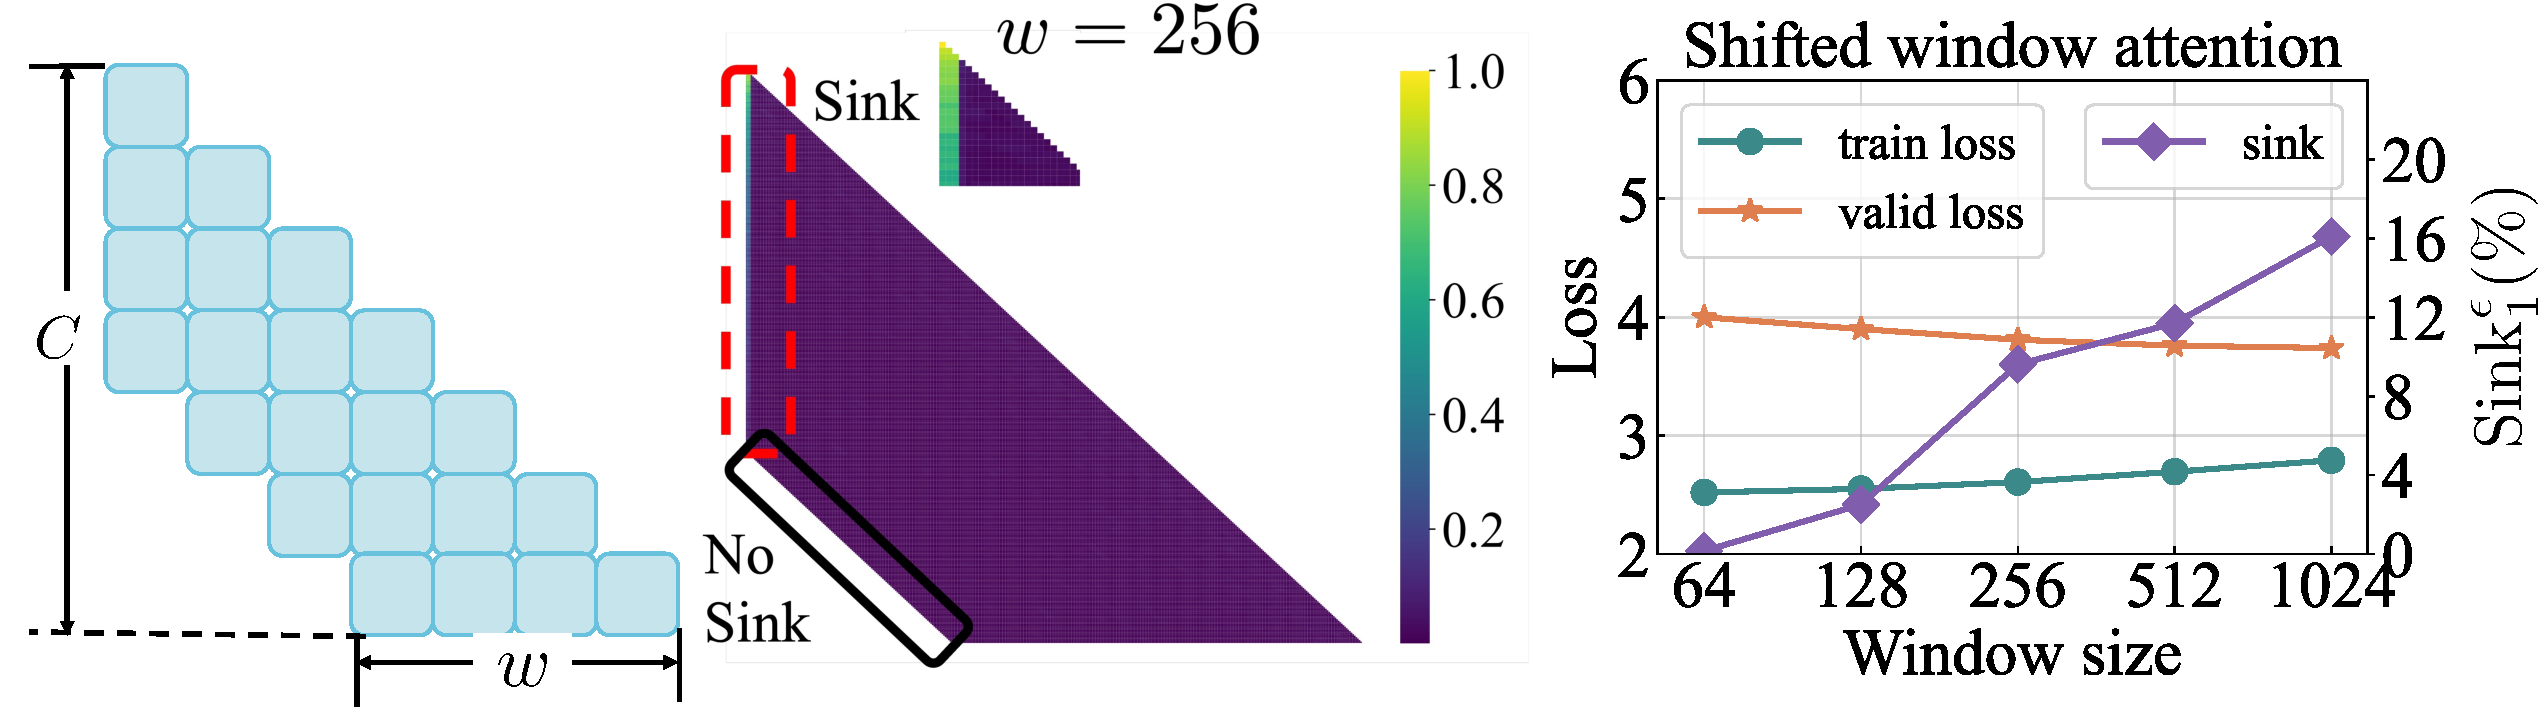
\includegraphics[width=\textwidth]{figures/window_attention.pdf}
\caption{(\emph{Left}) Shifted window attention pattern. (\emph{Middle}) In LMs with window attention, attention sink appears on the first token, but not on the ``first token'' within each window. (\emph{Right}) Attention sink tends to emerge when the window size is large enough.\looseness=-1 
}
\label{window}
\vspace{-0.2cm}
\end{figure}


\textbf{Prefix language modeling.} Since the first token is not predicted in the auto-regressive loss function, it could be considered as the prefix token. Then the original auto-regressive loss can be generalized into the formula $\mathcal{L}=\sum_{t=p+1}^C\log p_{\theta}(\boldsymbol{x}_t|\boldsymbol{x}_{p+1:t-1}\textrm{,}\,\boldsymbol{x}_{1:p})$, with the prefix length $p=1$. Motivated by \citet{wang2022language}, we consider $p>1$ and the casual mask visualized in Figure~\ref{data}(\emph{Left}). Although this design does not affect the emergence of attention sink, it shifts the sink position. In Figure~\ref{data}(\emph{Middle}), the attention sink only appears on one token. But it appears among these prefix tokens instead of on the first token only. Massive activations also appear on the corresponding sink token.\looseness=-1


% \begin{equation}
%     \mathcal{L}=\mathbb{E}_{\boldsymbol{X}\sim p_{\textrm{data}}}\left[\sum_{t=p+1}^C\log p_{\theta}(\boldsymbol{x}_t|\boldsymbol{x}_{p+1:t-1}\textrm{,}\,\boldsymbol{x}_{1:p})\right]
% \end{equation}



% \begin{table}[t]
% \begin{center}
% \begin{tabular}{l|ccccc}
% \toprule
% Unmasked tokens & 2 & 3 & 4 & 5 & 10 \\
% \midrule
% $\alpha_1$ (\%) & 4.96 & 8.47 & 3.05 & 1.80 & <1\\
% $\alpha_2$ (\%) & 9.89 & 6.97 & 8.88 & 7.30 & 2.50\\
% $\alpha_3$ (\%) & 3.37 & 2.08 & 4.59 & 4.62 & 4.15\\
% $\alpha_4$ (\%) & 1.5 & <1 & 2.26 & 2.35 & 3.90\\
% $\alpha_5$ (\%) & < 1 & <1 & <1 & 1.46 & 3.73\\
% % % \midrule
% % $\beta_1$ & 3.18 & 3.16 & 3.38 & 3.27 \\
% \bottomrule
% \end{tabular}
% \end{center}
% \vspace{-.2cm}
% \caption{Prefix Large Language Models.}
% \vspace{-.2cm}
% \label{tbl_decay_ema}
% \end{table}

\textbf{Shifted window attention.} Motivated by the shifted window attention adopted in Mistral-7B, we further explore the effects of window size on attention sink. With shifted window attention, the loss function becomes $\mathcal{L}=\sum_{t=2}^C\log p_{\theta}(\boldsymbol{x}_t|\boldsymbol{x}_{t-w:t-1})$, where $w$ refers to the window size. As shown in Figure~\ref{window}(\emph{Left}) and (\emph{Middle}), with shifted window attention, we find that if $t\leq w$, the $t$-th token can still ``look at'' the first token, and LMs still have attention sink on the first token. When $t>w$, the $t$-th token can only attend up to the $t-w+1$-th token. Although this token is the ``first token'' for the $t$-th token, typically it has no attention sink. We have similar observations in Mistral-7B. Additionally, from Figure~\ref{window}(\emph{Right}), smaller window size prevents the emergence of attention sink.\looseness=-1

\vspace{-0.1cm}
\begin{abox} % are we tired of takeaway boxes? :>
    \looseness -1 \textbf{Takeaways:} 1.~Weight decay encourages the emergence of attention sink. 2.~With prefix language modeling, attention sink appears among the prefix tokens rather than the first token only. 3.~With shifted window attention, attention sink appears on the ``absolute'', not the  ``relative'' first token. Smaller window size prevents the emergence of attention sink.
\end{abox}

% \begin{equation}
% \mathcal{L}=\mathbb{E}_{\boldsymbol{X}\sim p_{\textrm{data}}}\left[\sum_{t=2}^C\log p_{\theta}(\boldsymbol{x}_t|\boldsymbol{x}_{t-w:t-1})\right]
% \end{equation}

% \begin{table}[t]
% \caption{Attention sink tends to emerge when the window size is large enough. We use * to denote that $T$ is 32 instead of 64 when computing $\textrm{Sink}_1^{\epsilon}$.}
% \vspace{-.2cm}
% \begin{center}
% \begin{tabular}{l|cccccccc}
% \toprule
% Window size & 32 & 64 & 128 & 256 & 512 & 1024\\
% \midrule
% $\textrm{Sink}_1^{\epsilon}$(\%)  & \,\,\,0.80* & 0.16 & 2.51 & 9.61 & 11.70 & 16.10\\
% Valid loss & 4.11 & 4.00 & 3.90 & 3.81 & 3.76  & 3.74 \\
% \bottomrule
% \end{tabular}
% \end{center}
% \vspace{-.2cm}
% \label{window}
% \end{table}


% \begin{table}[t]
% \begin{center}
% \begin{tabular}{l|cccccccc}
% \toprule
% Window size &  64 & 128 & 256 & 512 & 1024\\
% \midrule
% $\textrm{Sink}_1^{\epsilon}$(\%)  &  0.16 & 2.51 & 9.61 & 11.70 & 16.10\\
% Valid loss & 4.00 & 3.90 & 3.81 & 3.76  & 3.74 \\
% \bottomrule
% \end{tabular}
% \end{center}
% \vspace{-.2cm}
% \caption{Window Attention}
% \vspace{-.2cm}
% \label{decay}
% \end{table}
